\documentclass[12pt]{article}
\usepackage[left=2cm,right=2cm,top=2cm,bottom=2cm,bindingoffset=0cm]{geometry}
\usepackage{fontspec}
\usepackage{polyglossia}
\usepackage{amssymb}
\setdefaultlanguage{russian}
\setmainfont[Mapping=tex-text]{CMU Serif}

\begin{document}
%% Весь этот текст можно удалить
%% ====== от сих =====
\begin{center}
  \LARGE Формальные языки 

  \Large домашнее задание до 23:59 09.03
\end{center}
\bigskip

\begin{enumerate}
  \item Минимизировать ДКА $(\{A, B, C, D, E\}, \{0, 1\}, \delta, A, \{ C, D \})$, где $\delta$ задана таблицей ниже, применив алгоритм минимизации. Приведите заполненную таблицу и порядок помещения пар в очередь.
  \begin{center} 
\begin{tabular}{c|c|c}
$\delta$ & $0$ & $1$ \\ \hline
$A$ & $B$ & $C$ \\
$B$ & $D$ & $E$ \\
$C$ & $B$ & $C$ \\
$D$ & $B$ & $C$ \\
$E$ & $D$ & $E$ \\
\end{tabular}
\end{center}
    \item Детерминизируйте следующий автомат, применив алгоритм Томпсона. Называйте состояния ДКА соответственно множеству состояний НКА ($\{ A, C, D \} \rightarrow ACD $).
    
        \begin{center} 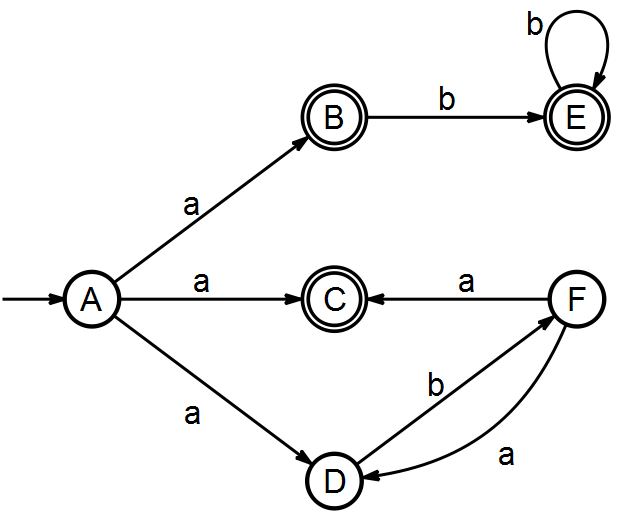
\includegraphics[width=0.5\linewidth]{../../2016_win/ElTech/2exdet.png} \end{center}
    \item Минимизируйте автомат, полученный в предыдущем задании. Покажите, что полученный автомат действительно минимален (построением таблицы, при помощи правых контекстов или словесной аргументацией)
\end{enumerate}  


%% ===== и до сих =====
\end{document}
